%------------------------------------------------------------
% Description : 
% Author      : taxus-d <iliya.t@mail.ru>
% Created at  : Thu Jan 12 14:26:18 MSK 2017
%------------------------------------------------------------
\documentclass[12pt,hardcopy]{../../../notes}
\usepackage{silence}
\WarningFilter{latex}{Reference}
\graphicspath{{../../img/}}

\begin{document}
\paragraph{Аксиоматическое определение вероятности}
\label{par:prob::ax}

\begin{defn}[$\sigma$-алгебра]\label{defn:prob::ax::sigmalg}
  Алгеброй $\mathcal A$ подмножеств множества $\Omega$ называется такой набор его подмножеств с
  заданными операциями объединения, пересечения и дополнения множеств, что
  \begin{enumerate}
    \item $\Omega \in \mathcal A$
    \item $X\in \mathcal A \Rightarrow \overline{X} \in \mathcal A$
    \item $X_1, X_2 \in \mathcal A \Rightarrow X_1 \cup X_2$
  \end{enumerate}

  Сигма-алгеброй подмножеств называется всё тоже самое, только можно объединять счётное число
  подмножеств.
\end{defn}
\begin{defn}[Вероятностное пространство]\label{defn:prob::ax::probspace}
  Рассмотрим упорядоченную тройку $(\Omega, \mathcal F, P)$, где
  \begin{description}
    \item[$\Omega$~---] Множество (элементарных исходов). Чисел, например.
    \item[$\mathcal F$~---] $\sigma$~--- алгебра подмножеств $\Omega$
    \item[$P$~---] Собственно, вероятность
  \end{description}
\end{defn}

\begin{defn}[Вероятность]\label{defn:prob::ax::probdef}
  $P\colon \mathcal F \to \R$ такая, что
  \begin{enumerate}
    \item $\forall\, A\;\: F(A) \geqslant 0$
    \item $\forall\, \{A_i\}\colon A_i \cap A_j = \varnothing 
      \;\; P\left(\bigcup_i A_i\right) = \sum_i P(A_i)$
    \item $P(\Omega) = 1$
  \end{enumerate}
  Как видно, сильно похоже на площадь. Что впрочем неслучано, вероятность~--- нормированная мера.
  Последнее условие как раз и означает нормированность. 
\end{defn}

\begin{defn}[Тривиальные события]\label{defn:prob::indep::triv}
  $\varnothing, \Omega$.
\end{defn}

\begin{prop}\label{prop:prob::ax::probprop}
  Свйоства вероятности:
  \begin{enumerate}
    \item $P(\varnothing) = 0$
    \item $0 \leqslant P(A) \leqslant 1$
    \item $ P(\overline{A}) = 1- P(A)$
    \item $ P(A\cup B) = P(A) + P(B) - P(A\cap B)$
  \end{enumerate}
\end{prop}
А это очень важное и будет в отдельном утверждении.
\begin{prop}[Непрерывность меры]\label{prop:prob::ax::cont}
  Пусть $A_1 \subset \cdots A_n \subset \cdot$, $\bigcup\limits_i A_i = A$. Тогда $P(A) =
  \lim\limits_{n\to \infty} P(A_n)$.
\end{prop}
\begin{itlproof}
  Пусть
  \begin{align*}
    B_1 &= A_1 \\
    B_2 &= A_2 \setminus A_1 \\
    \cdots&\cdots\cdots 
    \intertext{Тогда} 
    A &= \bigcup_{i=1}^\infty B_i;\; A_n = \bigcup_{i=1}^n B_n
    \intertext{Следовательно,}
    P(A) = \sum_{i=1}^\infty P(B_i) &= \lim_{n\to\infty} \sum_{i=1}^n P(B_i) = \lim_{n\to\infty}
    P(A_n)
  \end{align*}
  Всё работает, потому что в $\sigma$-алгебре можно объединять счётное число множеств.
\end{itlproof}

\paragraph{Формула полной вероятности}
\label{par:prob::compl}

\begin{defn}[Условная вероятность]\label{defn:prob::compl::condprob}
  Пусть $A, B \in \mathcal F$, $P(A) > 0$\note{ну мы же делим, нажо убедиться что неноль}. Тогда
  \[
    P(B \mid A) := \frac{P(B\cap A)}{P(A)} 
  \]
\end{defn}

\begin{prop}\label{prop:prob::compl::form}
  Пусть $\{A_i, H\} \subset \mathcal F$ и
  \begin{enumerate}
    \item $P(A_i) > 0$
    \item $A_i \cap A_j = \varnothing$
    \item $\bigcup_i A_i = \Omega$
  \end{enumerate}
  (полная группа/система событий). Тогда
  \[
    P(H)=\sum_i P(A_i)\cdot P(H\mid A_i)
  \]
\end{prop}

\paragraph{Теорема Байеса}
\label{par:prob::bayes}

\begin{thrm}\label{thrm:prob::bayes}
  Пусть $A_i$~--- полная система событий, $H\in \mathcal F\colon P(H)>0$. Тогда 
  \[
    P(A_k \mid H) = \frac{P(A_k)\cdot P(H \mid A_k)}{\sum_i P(A_i)\cdot P(H\mid A_i)} 
  \]
\end{thrm}

\paragraph{Независимые события}
\label{par:prob::indep}

\begin{defn}\label{defn:prob::indep::indep}
  Пусть $A, B\in \mathcal F$. Они назывыются независимыми, если 
  \[
    P(A\cap B) = P(A)\cdot P(B)
  \]
\end{defn}

\begin{prop}\label{prop:prob::indep::cond}
  События $A,B$ независимы $ \Leftrightarrow $ $P(A\mid B) = P(A) \lor P(B\mid A) = P(B)$ (в
  зависимости от того, что определено, вдруг там ноль где-нибудь).
\end{prop}
\begin{prop}\label{prop:prob::indep::zerodep}
  Если $A,B$ несовместны, то нетривиальные $A,B$~--- зависимы.
\end{prop}

\begin{defn}\label{defn:prob::indep::pair}
  Случайные величины $\{X_i\}$ попарно независимы, если 
  \[\forall\,i,j\;\; P(X_i\cap X_j) = P(X_i)\cdot P(X_j)\]. 
\end{defn}
\begin{defn}\label{defn:prob::indep::set}
  Случайные величины $\{X_i\}_{i=1}^n$ независимы по совокупности , если \[
    \forall\,\{i_k\mid i_k,k \in (\Z\cap[1;n]) \}\;\; P\left(\bigcap_{i_k} X_{i_k}\right) 
    = \prod_{i_k}  P(X_{i_k})
  \] 
\end{defn}
\begin{rem}\label{rem:prob::indep::bern}
  Определения \ref{defn:prob::indep::set} и \ref{defn:prob::indep::set} правда разные.
  Конечно попарная независимость следует из независимости по совокупности, но обратное неверно.
\end{rem}
\begin{exmp}\label{exmp:stat::shwartz::bern}
  Тетраэдр Бернштейна:
  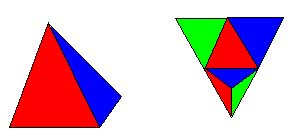
\includegraphics[scale=0.5]{berntetragon}. Здесь вероятность выпадения всех 3 цветов~--- $\lfrac
  1 4$, а через попарные~--- $\lfrac 1 8$
\end{exmp}

\paragraph{Случайные величины и их распределения}
\label{par:prob::randscal}

\begin{defn}[Случаная величина]\label{defn:prob::randscal::randscal}
  Случайной величиной назовём произвольное хорошее отображение $X\colon \Omega \to \R$.
  
  \begin{itaux}\label{rem:prob::randscal::meas}
    Тут нужно бы сказать про измеримость, это потребуется, чтобы говорить о вероятности попадания в
    интервал на прямой. Так что \[
      X\colon \bigl(X^{-1} (B) =\{\omega \mid X(\omega)\in B\}\bigr)\in \mathcal F,
    \]
    где $B$~--- борелевское множество
  \end{itaux}

\end{defn}

\begin{defn}\label{defn:prob::randscal::inborel}
  Пусть $B\subset \R$, $B$~--- промежуток, или дополнение в нему (борелевское множество).\note{тут
  вроде концы могут входить, так что точка~--- тоже борелевское множество.}
  \[
    P(X\in B) = P(\{\omega \mid X(\omega) \in B\})
  \]
\end{defn}

\begin{defn}\label{defn:prob::randscal::disc}
  Случайная величина называется дискретной, если
  \[
    \exists\,(\{a_i\} \sim \N)\colon \left( \sum_{i} P(X = a_i) = 1 \right)
  \]
  то есть 
  \[
    P(X\in B) = \sum_{\{i\mid a_i\in B\}} p_i, \; p_i = P(X = a_i)
  \]
\end{defn}
\begin{defn}\label{defn:prob::randscal::cony}
  Случайная величина называется непрерывной, если
  \[
    \exists\,(f_X\colon B\to \R )\colon \left( P(X\in B) = \int_{B} f_X(x)\, \del x \right)
  \]
\end{defn}
\begin{defn}[Распределение случайной величины]\label{defn:prob::randscal::distr}
  $F(B) = P(X \in B)$
\end{defn}

\begin{exmp}[К непрерывному распределению]\label{exmp:prob::randscal::cont}
  Пусть $X(\omega) = \omega$, $B = (0,1)$, $\Omega = (-1;1)$. Выберем  $f_X \equiv \frac{1}{2}$.
  \begin{align*}
    F(B) = P(X\in B) = P(\{\omega \mid \omega \in (0,1)\}) = P\bigl((0,1)\bigr) = \tfrac{1-0}{1+1}
    = \tfrac{1}{2} \\
    F(B) = \int_{(0,1)} \tfrac{1}{2}\, \del x  = \tfrac{1-0}{2} = \tfrac{1}{2}
  \end{align*}
  Это всё верно, потому что на множестве интервалов вероятность~--- нормированная длина интервала.
\end{exmp}

\begin{defn}[Функция распределения]\label{defn:prob::randscal::distrfun}
  \[
    F_X\colon \R\to [0;1] \colon\; F_X(x) = P(X < x) = P(\{\omega \mid X(\omega) < x \})
  \]
\end{defn}

\begin{prop}\label{prop:prob::randscal::distrfun}
  Про $F(x)$ верно следущее:
  \begin{enumerate}
    \item $F\displaystyle\uparrow \R$
    \item $\displaystyle\lim_{x\to -\infty}F(x) = 0$
    \item $\displaystyle\lim_{x\to +\infty}F(x) = 1$
    \item $\displaystyle\lim_{x\to x_0-0}F(x) = F(x_0)$
  \end{enumerate}
\end{prop}

\begin{prop}\label{prop:prob::randscal::inv}
  Верно и обратное: если существует функция с  указанными свойствами, под неё найдётся случайная
  величина. 
\end{prop}
% \begin{itlproof}
%   Вроде борелевская сигма-алгебра покатит.
%   X = sup 
% \end{itlproof}

\begin{rem*}\label{rem*:prob::randscal::delta}
  Если рассматривать обобщённые функции, то любое распределение запишется как
  \[
    \int_{-\infty}^x f_X(u)\,\del u
  \]
\end{rem*}
\paragraph{Моменты случайных величин}
\label{par:prob::moments}

\begin{defn}\label{defn:prob::moments::exp}
  Пусть $X$~--- случайная величина, \[
    \int_{-\infty}^{\infty} |x| f_X(x)\, \del x < \infty 
  \]
  Тогда 
  \[
    \langle x \rangle \equiv \bar x \equiv \Exp X = \int_{-\infty}^{\infty} x f_X(x)\, \del x
  \]
\end{defn}

\begin{prop}\label{prop:prob::moments::expprop}
  Свойства матожидания:
  \begin{enumerate}
    \item $\Exp < \infty$
    \item $\Exp(a X + b Y) = a\Exp X + b\Exp Y$
    \item $P(X \geqslant 0) = 1 \Rightarrow \Exp X \geqslant 0 $
    \item $\begin{cases}
      P(X \geqslant 0) = 1 \\
      \Exp X = 0
    \end{cases}\Rightarrow P(X= 0) =1  $
    \item если $X,Y$~--- независимы, то $\Exp (XY) = \Exp X \cdot \Exp Y$
  \end{enumerate}
\end{prop}

\begin{defn}\label{prop:prob::moments::mom}
  Момент $k$-ого порядка относительно начала $a$:
  \[
    \lambda_{k,a} = \int_{-\infty}^{\infty} (x-a)^k f(x)\, \del x
  \]
  (если есть абсолютная сходимость)
\end{defn}
% dedicated to lisp fans
{\defn\label{defn:prob::moments::zer} Начальный  момент: {$\nu_k =\lambda_{k,0}$}}
{\defn\label{defn:prob::moments::cen} Центральный  момент: {$\mu_k =\lambda_{k,\bar x}$}}

{\prop\label{prop:prob::moments::conn} $\displaystyle\nu_k=\sum_{i=0}^k C_k^i a^i \,\lambda_{k-i,a}$}

\begin{defn}[Дисперсия]\label{defn:prob::moments::var}
  $\Var X = \Exp (X-\Exp X)^2$, $\sigma = \sqrt{\Var X}$~--- среднеквадратичное отклонение.
\end{defn}

\begin{prop}\label{prop:prob::moments::varprop}
  \item $\Var(a X + b Y) = a^2 \Var X + b^2 \Var Y$
  \item если $X,Y$~--- независимы, то $\Var (XY) = \Var X \cdot \Var Y$
  \item $\Var(X+C) = \Var X$
\end{prop}

\paragraph{Характеристическая функция}
\label{par:prop::charfun}

\begin{defn}[Характеристическая функция]\label{defn:prob::moments::charfun}
  $\displaystyle \Phi(t) = \Exp e^{itx}$
\end{defn}

\begin{prop}\label{prop:prob::charfun::charfun}
  Свойства характеристической функции:
  \begin{enumerate}
    \item Всегда существует и $|\Phi(t)| \leqslant 1$.
    \item $f(x) = \dfrac{1}{2\pi} \dint_{-\infty}^\infty e^{-itx} \Phi(t) \,\del t $
    \item $\Phi_{a + Xb} (t) = e^{ita} \Phi_X (tb)$
    \item Если $X,Y$~--- независимы, то $\Phi_{X+Y}(t)=  \Phi_X(t) \Phi_Y(t)$
    \item Если $\Exp |X|^n < \infty$, то $\Phi^{(k)}(0)=  i^k \Exp X^k$
  \end{enumerate}
\end{prop}
\begin{defn}[Сходимость по распределению]\label{defn:prob::charfun::distconv}
  $X_n \xrightarrow{d} X \Leftrightarrow F_n(x) \to F(x)$ 
\end{defn}
\begin{thrm}[О непрерывном соответствии]\label{thrm:prob::charfun::contchar}
  $X_n \xrightarrow{d} X \Leftrightarrow \Phi_{X_n} (t)
  \underset{t}{\rightrightarrows} \Phi_X(t)$.
  Здесь на самом деле всё сложно. В разных книжках пишут равномерную сходимость на разных
  интервалах. У нас вроде было на всей вещественной прямой, но тогда это слишком сильное
  утверждение. К слову так же в \cite{chernova1} и \cite{shiriaev}. А вот в \cite{msu} требуют
  только сходимости в каждом конечном интервале. Можно взять экспоненту, и понять, что эти
  условия разные. 
\end{thrm}
\paragraph{Теорема Муавра-Лапласа}
\label{par:prob::laplace}

\end{document}
% vim:wrapmargin=3
